%!TEX root = ../main.tex

\section{Supplemental Material}

The Di Blasi kinetics were put to use in a batch reactor model to investigate the time scales associated with the reaction mechanisms. Figure \ref{fig:batch-blasi} is an overview of the biomass conversion and pyrolysis yields using the Di Blasi kinetics in a batch reactor at 773.15 K (500$^\circ$C). At this temperature, without the effects of secondary reactions, the kinetics offer a maximum achievable tar yield of 78\% within 5 seconds. However, if secondary reactions occur during the entire pyrolysis process then a maximum tar yield of only 53\% is possible. Modifying the pre-factor term for reaction 4 by a factor of 0.2, decreases the gas yield while increasing tar and char yields. The Di Blasi kinetics suggest that minimizing the extent of secondary reactions is critical to producing the maximum possible tar yield.

A range of reaction temperatures were applied to the Di Blasi kinetics in the batch reactor model as shown in Figure \ref{fig:batch-blasi-temps}. The kinetics suggest that temperature can increase the rate of primary tar production while decreasing devolatilization time. When secondary reactions occur during the entire pyrolysis process, maximum tar yields are realized at higher temperatures but with shorter residence times. These results suggest that if secondary reactions are minimized then maximum tar yield can be achieved within an appropriate residence time.

\begin{figure}[H]
    \centering
    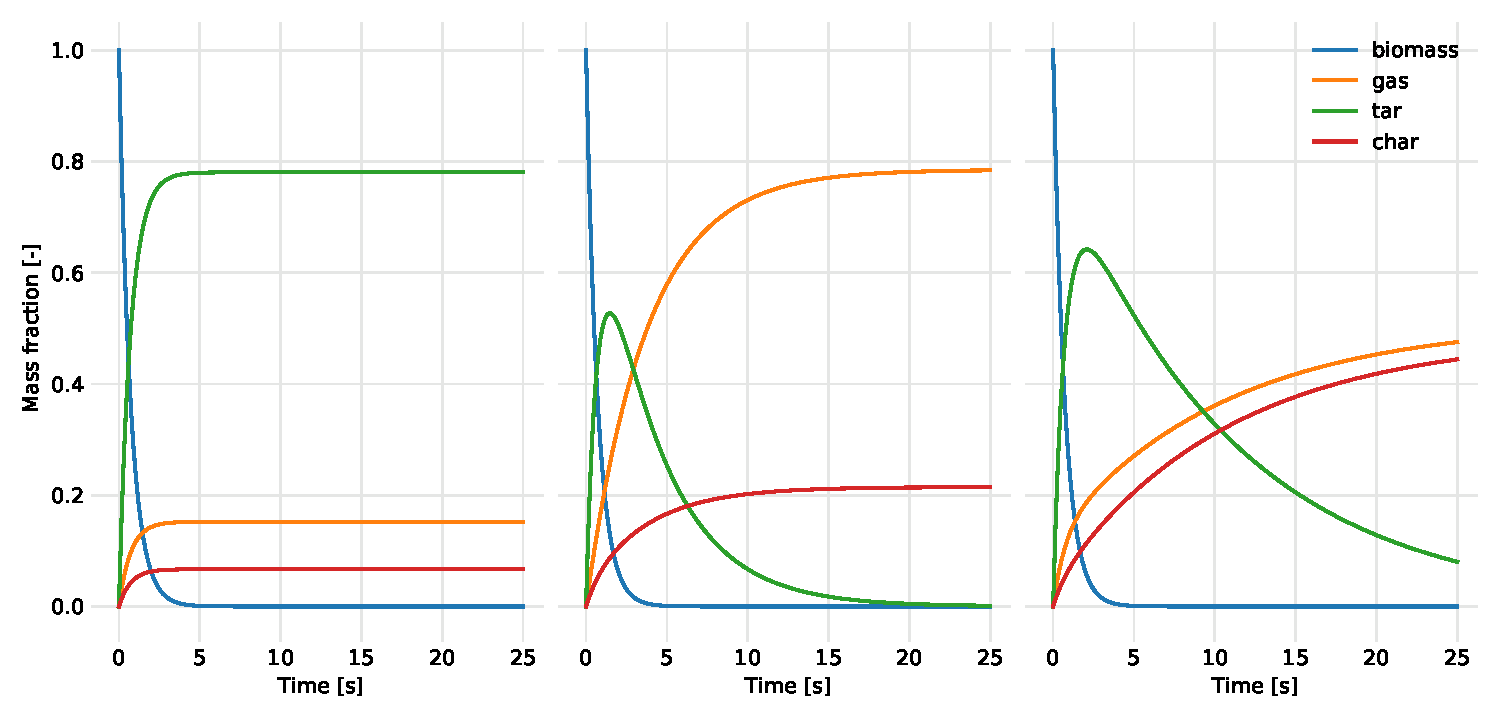
\includegraphics[width=\textwidth]{batch-blasi.pdf}
    \caption{Biomass conversion and product yields in a batch reactor model at 773.15 K (500$^\circ$C) according to the Di Blasi kinetic reactions. Primary reactions only (left). Primary and secondary reactions (center). Primary and secondary reactions using modified reaction 4 (right).}
    \label{fig:batch-blasi}
\end{figure}

\begin{figure}[H]
    \centering
    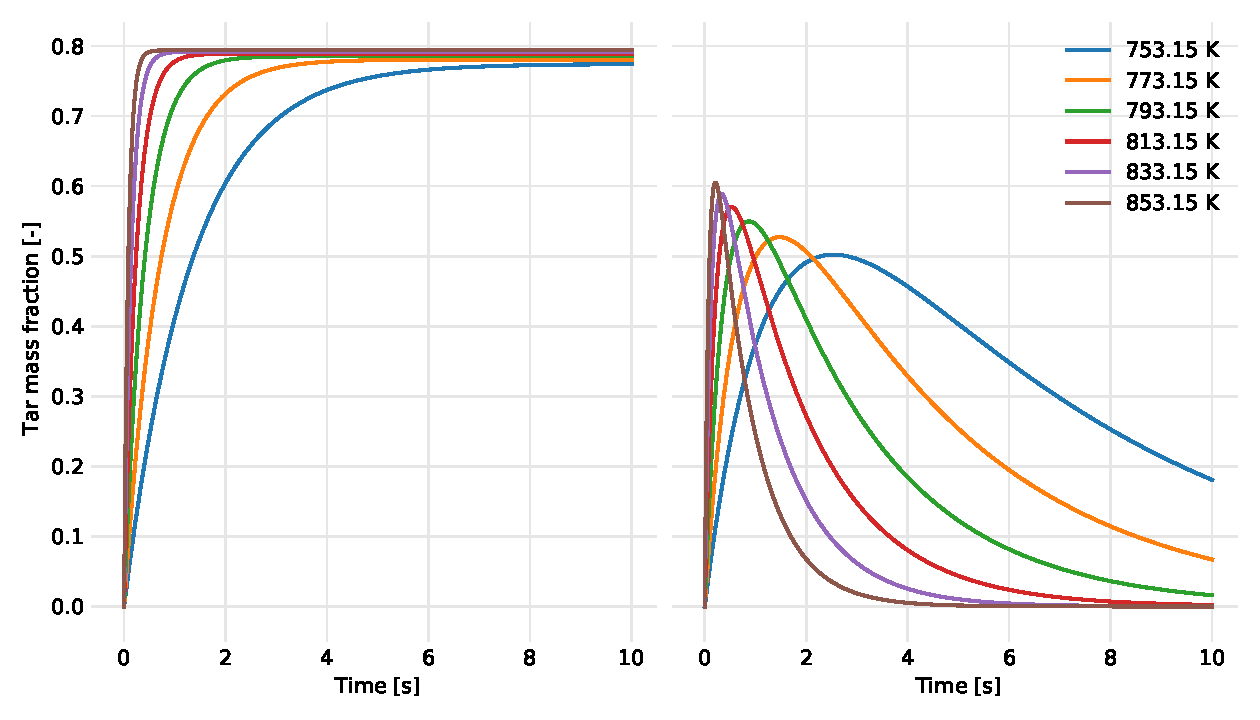
\includegraphics[width=\textwidth]{batch-blasi-temps.pdf}
    \caption{Tar yields for reaction temperatures of 753.15--853.15 K (480--580$^\circ$C) using the Di Blasi kinetics in a batch reactor model. Results shown for primary tar (left) along with primary and secondary tar (right).}
    \label{fig:batch-blasi-temps}
\end{figure}
